\documentclass{article}
\usepackage[T1]{fontenc}
\usepackage{lmodern}
\usepackage[utf8]{inputenc}
\usepackage[british]{babel}
\usepackage{geometry}
\usepackage{color}
\usepackage{amsthm}
\usepackage{amsmath,amssymb}
\usepackage{graphicx}
\usepackage{mathtools}
\usepackage{listings}
\usepackage{newlfont}
\usepackage{tikz-cd}
\usepackage{faktor}

\newcommand{\numberset}{\mathbb}
\newcommand{\N}{\numberset{N}}
\newcommand{\Z}{\numberset{Z}}
\newcommand{\R}{\numberset{R}}
\newcommand{\Q}{\numberset{Q}}
\newcommand{\C}{\numberset{C}}
\newcommand{\K}{\numberset{K}}
\newcommand{\F}{\numberset{F}}
\newcommand{\n}{\mathcal{N}}
\newcommand{\aid}{\mathfrak{a}}
\newcommand{\bid}{\mathfrak{b}}
\newcommand{\pid}{\mathfrak{p}}
\newcommand{\qid}{\mathfrak{q}}
\newcommand{\mi}{\mathfrak{m}}
\newcommand{\I}{\mathbb{I}}
\newcommand{\V}{\mathbb{V}}

\DeclareMathOperator{\Ima}{Im}

\newcommand{\exercise}[1]{\noindent {\bf Exercise #1}}

\begin{document}

\title{Algebraic Topology 1 - Assignment 3}

\author{M. Durante, 2303760, Leiden University\\T.A.H.A Quemener, 2304252, Leiden University}

\maketitle


\exercise{1}

\begin{align*}
		G:\R^2\times I & \rightarrow R^2 \\
		((x,y),t) & \mapsto (x+t,y)
\end{align*}

This map is continuous and $G(-,0)=f,\ G(-,1)=g$, hence it is a homotopy among the two maps.

\begin{align*}
		\sigma:\Delta^2 & \rightarrow \R^2 \\
		(1-t-h,t,h) & \mapsto (t,h) \\
		f_*\sigma:\Delta^2 & \rightarrow \R^2 \\
		(1-t-h,t,h) & \mapsto (t,h) \\
		g_*\sigma:\Delta^2 & \rightarrow \R^2 \\
		(1-t-h,t,h) & \mapsto (1+t,h)
\end{align*}

\begin{figure}
		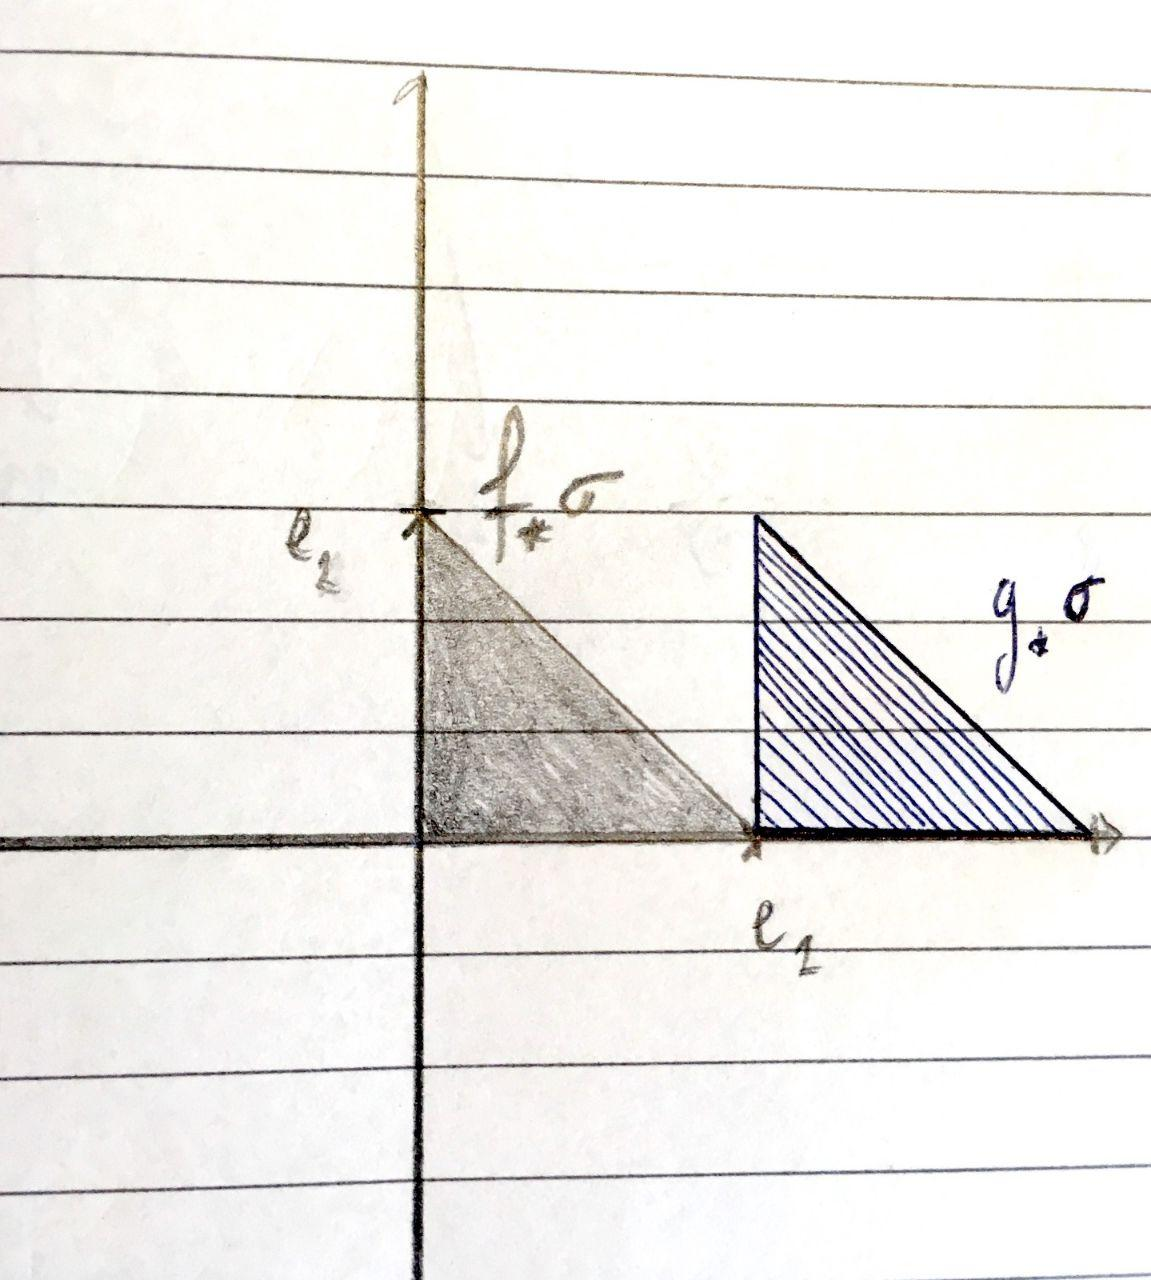
\includegraphics[width=4cm]{pic1ass3at1.jpg}
		\caption{Representation of these singular simpleces.}
\end{figure}

To find $P_2(\sigma)$, first we shall compute the summands explicitly.
\begin{align*}
		\sigma\sigma_0:\Delta^3 & \rightarrow\R^2 \\
		(1-t-h-k,t,h,k) & \mapsto (h,k) \\
		\sigma\sigma_1:\Delta^3 & \rightarrow\R^2 \\
		(1-t-h-k,t,h,k) & \mapsto (t+h,k) \\
		\sigma\sigma_2:\Delta^3 & \rightarrow\R^2 \\
		(1-t-h-k,t,h,k) & \mapsto (t,h+k)
\end{align*}

Consider $G_*:C(\R^2\times I,A)_3\rightarrow C(\R^2,A)_3$. This is defined as $G_*(af)=aG(f)$, for $a\in A$ and $f\in S(\R^2\times I)_3$.

Now, given the definition of $\alpha_i$, considering the 3-singular simplex $(f,\alpha_i):\Delta^3\rightarrow\R^2\times I$ sending $P$ to $(f(P),\alpha_i(P))$, we compute $G_*(1(\sigma\sigma_i,\alpha_i))=1G(\sigma\sigma_i,\alpha_i)$ for $i=0,1,2$ remembering that, for $j\leq i$, $G(\sigma\sigma_i,\alpha_i)(j)=G(\sigma\sigma_i(j),0)=f\sigma\sigma_i(j)$, while for $j>i$ we get that $G(\sigma\sigma_i,\alpha_i)(j)=G(\sigma\sigma_i(j),1)=g\sigma\sigma_i(j)$.

\begin{align*}
		G(\sigma\sigma_0,\alpha_0):\Delta^3 & \rightarrow\R^2 \\
		(1-t-h-k,t,h,k) & \mapsto (t+2h+k,k) \\
		G(\sigma\sigma_1,\alpha_1):\Delta^3 & \rightarrow\R^2 \\
		(1-t-h-k,t,h,k) & \mapsto (t+2h+k,k) \\
		G(\sigma\sigma_2,\alpha_2):\Delta^3 & \rightarrow\R^2 \\
		(1-t-h-k,t,h,k) & \mapsto (t+k,h+k)
\end{align*}

Now, $P_2(\sigma)=\sum_{i=0}^2 (-1)^iG_*(1(\sigma\sigma_i,\alpha_i))=1G(\sigma\sigma_2,\alpha_2)$.

The singular simplex, combined with the ones in the previous pictures, creates what we may see in 3 dimensions as a prism, with the previous $2$-singular simpleces acting as triangular bases and this $3$-singular simplex $P_2(\sigma)$ being the volume filling it up.

The reason why the two singular simpleces $f_*\sigma$ and $g_*\sigma$ differ by more than a boundary and this doesn't cause any problem w.r.t. the induced homomorphisms between homology groups is that $\sigma$ (and, by the similar computations, $f_*\sigma=\sigma$ and $g_*\sigma$) doesn't belong to $\ker(\partial_2)$ and $H_2(\R^2,A)=\ker(\partial_2)/\Ima(\partial_3)$.
\begin{align*}
		\sigma\delta_0:\Delta^1 & \rightarrow \R^2 \\
		(1-t,t) & \mapsto (1-t,t) \\
		\sigma\delta_1:\Delta^1 & \rightarrow \R^2 \\
		(1-t,t) & \mapsto (0,t) \\
		\sigma\delta_2:\Delta^1 & \rightarrow \R^2 \\
		(1-t,t) & \mapsto (t,0)
\end{align*}

Clearly, $1\sigma\delta_0$, $1\sigma\delta_1$ and $1\sigma\delta_2$ are linearly independent, hence $\partial_2(1\sigma)\neq 0$. Furthermore, $\partial_2(\sigma),\partial_2(f_*\sigma)$ and $\partial_2(g_*\sigma)$ lie in $\Ima(\partial_2)$, thus they belong to the same homology class in $H_1(\R^2,A)$.

~\\
~\\
\exercise{2}

We can see any $n$-simplex as an object in $\R^n$: to do this we may consider the restriction to $\Delta^n$ of the projection from $\R^{n+1}$ to $\R^n$ omitting the first coordinate, which on $\Delta^n$ is uniquely determined by the others, and in this way obtain an homeomorphism between the actual $n$-simplex and its projection. Indeed, the projection map is an identification, hence, being injective on $\Delta^n$, it establishes a bijection between $\Delta^n$ and $\pi(\Delta^n)$, and therefore an homeomorphism between these two subspaces.

This projected $n$-simplex has non-empty interior since it contains an open ball, the one centered at its baricenter and of radius $\frac{1}{4n^2}$, and it is compact (closed and limited). Furthermore, as we will show, it is convex.

Indeed, let $P,Q\in\Delta^n$. Then, seeing the $n$-simplex again in $\R^n$, $P=\sum_{i=1}^n t_ie_i$ and $Q=\sum_{i=1}^n h_ie_i$. Now, given $\lambda\in I$, consider the linear combination $\lambda P+(1-\lambda)Q=\lambda(\sum_{i=1}^n t_ie_i)+(1-\lambda)(\sum_{i=1}^n h_ie_i)$. We observe that $\lambda\sum_{i=1}^n t_i+(1-\lambda)\sum_{i=1}^n h_i\leq \lambda+(1-\lambda)=1$, thus $\lambda P+(1-\lambda)Q$ belongs to our projected $\Delta^n$.

By~\cite[prop. 16.4]{bred}, this means that the projected $\Delta^n$ (and therefore $\Delta^n$ itself) is homeomorphic to a closed ball in $\R^n$, $B^n$.

Now, since all closed balls in the same space $\R^n$ are homeomorphic among them, we shall consider the unit balls centered at the origin.

Now, suppose that we have an homeomorphism between $\Delta^{19}$ and $\Delta^{18}$. Then, this induces an homeomorphism $B^{19}\xrightarrow{f} B^{18}$. Let us remove from $B^{19}$ any interior point $P$. Our homeomorphism will induce an homeomorphism $g:=f_{|B^{19}\setminus\{P\}}:B^{19}\setminus\{P\}\rightarrow B^{18}\setminus\{f(P)\}$.

We will show that, if $f(P)$ is interior, they are homotopically equivalent respectively to $S^{18}$ and $S^{17}$ by exhibiting the following retraction:
\begin{align*}
		H:B^n\setminus\{P\}\times I & \rightarrow B^n\setminus\{P\} \\
		(x,t) & \mapsto tx+(1-t)\frac{x-P}{||x-P||}
\end{align*}
$H(-,0)=Id_{B^n\setminus\{P\}}$ and $\Ima(H(-,1))=S^{n-1}$, hence, since $H$ is continuous (it is obtained through products and sum of continuous functions), it is the desired retraction.

By homotopic equivalence, it follows that, chosen $A\not\cong 0$, $H_k(B^n\setminus\{P\},A)=H_k(S^{n-1},A)$. As we know, for $k\neq n-1$ this is the trivial group, while for $k=n-1$ it is isomorphic to $A$, hence $H_{18}(S^{18},A)\not\cong H_{18}(S^{17},A)$.

On the other hand, if $f(P)$ belongs to $\partial B^{18}$, the following retraction shows that $B^{18}\setminus\{f(P)\}$ is homotopically equivalent to a point:
\begin{align*}
		H':B^n\setminus\{f(P)\}\times I & \rightarrow B^n\setminus\{f(P)\} \\
		(x,t) & \mapsto tx
\end{align*}
This map is clearly continuous and $H'(-,0)=Id_{B^n\setminus\{f(P)\}}$, $\Ima(H'(-,1))=\{0\}$. Again, by homotopic equivalence, $H_n(B^n\setminus\{f(P)\},A)$ is isomorphic to $A$ if $n=0$ and it is trivial otherwise, hence $H_0(B^{18}\setminus\{f(P)\},A)\not\cong H_0(S^{18},A)$.

Since the homology groups are invariant under homeomorphism, the two spaces we obtained can't be homeomorphic, thus the original homeomorphism between the two simpleces doesn't exist.

\begin{thebibliography}{9}
		\bibitem{bred}
				G.E. Bredon,
				\textit{Topology and Geometry},
\end{thebibliography}

\end{document}
